\documentclass[12pt]{report}
\usepackage[utf8]{inputenc}
\usepackage[russian]{babel}
%\usepackage[14pt]{extsizes}
\usepackage{listings}
\usepackage{graphicx}
\usepackage{amsmath,amsfonts,amssymb,amsthm,mathtools} 
\usepackage{pgfplots}
\usepackage{filecontents}
\usepackage{indentfirst}
\usepackage{eucal}
\usepackage{enumitem}
\frenchspacing

\usepackage{indentfirst} % Красная строка


\usetikzlibrary{datavisualization}
\usetikzlibrary{datavisualization.formats.functions}

\usepackage{amsmath}



% Для листинга кода:
\usepackage{caption}
\DeclareCaptionFont{white}{\color{white}}
\DeclareCaptionFormat{listing}{\colorbox{white}{\parbox{\textwidth}{#1#2#3}}}
\captionsetup[lstlisting]{format=listing,justification=raggedright}

\lstset{ %
	language=C++,                 % выбор языка для подсветки
	basicstyle=\small\sffamily, % размер и начертание шрифта для подсветки кода
	keywordstyle=\color{blue},
	numbers=left,               % где поставить нумерацию строк (слева\справа)
	numberstyle=\tiny,           % размер шрифта для номеров строк
	stepnumber=1,                   % размер шага между двумя номерами строк
	numbersep=5pt,                % как далеко отстоят номера строк от подсвечиваемого кода
	showspaces=false,            % показывать или нет пробелы специальными отступами
	showstringspaces=false,      % показывать или нет пробелы в строках
	showtabs=false,             % показывать или нет табуляцию в строках
	frame=single,              % рисовать рамку вокруг кода
	tabsize=2,                 % размер табуляции по умолчанию равен 2 пробелам
	captionpos=t,              % позиция заголовка вверху [t] или внизу [b] 
	breaklines=true,           % автоматически переносить строки (да\нет)
	breakatwhitespace=false, % переносить строки только если есть пробел
	escapeinside={\#*}{*)}   % если нужно добавить комментарии в коде
}

\usepackage[left=2cm,right=2cm, top=2cm,bottom=2cm,bindingoffset=0cm]{geometry}
% Для измененных титулов глав:
\usepackage{titlesec, blindtext, color} % подключаем нужные пакеты
\definecolor{gray75}{gray}{0.75} % определяем цвет
\newcommand{\hsp}{\hspace{20pt}} % длина линии в 20pt
% titleformat определяет стиль
\titleformat{\chapter}[hang]{\Huge\bfseries}{\thechapter\hsp\textcolor{gray75}{|}\hsp}{0pt}{\Huge\bfseries}


% plot
\usepackage{pgfplots}
\usepackage{filecontents}
\usetikzlibrary{datavisualization}
\usetikzlibrary{datavisualization.formats.functions}

\begin{document}
	\def\contentsname{Содержание}
	\def\refname{Список литературы}
	\thispagestyle{empty}
	\begin{titlepage}
		\noindent \begin{minipage}{0.15\textwidth}
			
\includegraphics[width=\linewidth]{b_logo}
		\end{minipage}
		\noindent\begin{minipage}{0.9\textwidth}\centering
			\textbf{Министерство науки и высшего образования Российской Федерации}\\
			\textbf{Федеральное государственное бюджетное образовательное учреждение высшего образования}\\
			\textbf{~~~«Московский государственный технический университет имени Н.Э.~Баумана}\\
			\textbf{(национальный исследовательский университет)»}\\
			\textbf{(МГТУ им. Н.Э.~Баумана)}
		\end{minipage}
		
		\noindent\rule{18cm}{3pt}
		\newline\newline
		\noindent ФАКУЛЬТЕТ $\underline{\text{«Информатика и системы управления»}}$ \newline\newline
		\noindent КАФЕДРА $\underline{\text{«Программное обеспечение ЭВМ и информационные технологии»}}$\newline\newline\newline\newline\newline
		
		
		\begin{center}
			\noindent\begin{minipage}{1.3\textwidth}\centering
				\Large\textbf{  Отчет по лабораторной работе №4}\newline
				\textbf{по дисциплине "Анализ алгоритмов"}\newline\newline
			\end{minipage}
		\end{center}
		
		\noindent\textbf{Тема} $\underline{\text{Параллельный поворот фигуры}}$\newline\newline
		\noindent\textbf{Студент} $\underline{\text{Петрова А.А.}}$\newline\newline
		\noindent\textbf{Группа} $\underline{\text{ИУ7-56Б}}$\newline\newline
		\noindent\textbf{Оценка (баллы)} $\underline{\text{~~~~~~~~~~~~~~~~~~~~~~~~~~~}}$\newline\newline
		\noindent\textbf{Преподаватели} $\underline{\text{Волкова Л.Л.}}$\newline\newline\newline
		
		\begin{center}
			\vfill
			Москва~---~\the\year
			~г.
		\end{center}
	\end{titlepage}
	
	
	\tableofcontents
	
	\newpage
	\chapter*{Введение}
	\addcontentsline{toc}{chapter}{Введение}
	Многопоточность - это специализированная форма многозадачности, и многозадачность - это функция, которая позволяет вашему компьютеру одновременно запускать две или несколько программ. В общем, существует два типа многозадачности: основанные на процессах и потоки \cite{wil}.
	
	Многозадачность на основе процессов управляет одновременным выполнением программ. Многозадачность на основе потоков связана с одновременным выполнением частей одной и той же программы.
	
	Многопоточная программа содержит две или несколько частей, которые могут запускаться одновременно. Каждая часть такой программы называется потоком, и каждый поток определяет отдельный путь выполнения.

	
	Целью данной лабораторной работы являются изучение и реализация многопоточности на основе алгоритмов компьютерной графики, в частности алгоритма поворота двумерной фигуры, представленной в виде массива
	точек.
	\newline
	
	Для достижения поставленной цели необходимо выполнить следующие задачи:
	\begin{itemize}
		\item изучить понятие параллельных вычислений;
		\item реализовать последовательный и параллельный алгоритмы поворота фигуры;
		\item сравнить временные характеристики реализованных алгоритмов экспериментально. 
	\end{itemize}
	
	\chapter{Аналитическая часть}
	
	В этом разделе будет проанализирована предметная область, установлена актуальность задачи, а также будет рассмотрен алгоритм задачи, которая будет подвергнута распараллеливанию.
	
	Задача поворота фигуры, представленной в виде массива точек в двумерном растре, является весьма актуальной, т.к. компьютерная графика стала неотъемлемой частью повседневной интернет-жизни человека, и существует потребность в быстром рендеринге изображения, например, при
	анимации поворота фигуры на двумерном растре. Как известно, в экранной плоскости изображение представляет из себя набор пикселей (точек). Очевидно, что какая-либо фигура - это тоже набор точек экранной плоскоти, и для поворота фигуры требуется над каждой ее точкой произвести
	преобразование для получения новой позиции.
	
	Если использовать один поток для рендеринга изображения, то при большом количестве и сложности фигур изображение будет генерироваться ощутимо долго, что будет приносить человеку дискомфорт при восприятии, однако если распараллелить этот процесс, т.е. параллельно генерировать части изображения (т.к. эта операция выполняется независимо для каждой точки), то это может дать коллосальной прирост производительности.
	
	\section{Алгоритм поворота точек на плоскости}
	
	Пусть необходимо повернуть точку $P(x,y)$ вокруг начала координат $O$ на угол $\phi$. Изображение новой точки обозначим $P'(x',y')$. Всегда существуют четыре числа $a, b, c, d$ такие, что новые координаты могут быть
	вычислены по значениям старых координат из следующей системы уравнений:
	
	\begin{equation}
		\label{eq1}
		\begin{cases}
			x'=a \cdot x+b \cdot y\\
			y'=c \cdot x+d \cdot y
		\end{cases}
	\end{equation}
	
	Для получения значений $a, b, c, d$ рассмотрим точку $P(x, y) = (1, 0)$. Полагая $x = 1$ и $y = 0$ в уравнении \ref{eq1}, получим:
	
	\begin{equation}
		\begin{cases}
			x'=a\\
			y'=c
		\end{cases}
	\end{equation}
	
	Но в этом простом случае, значения $x'$ и $y'$ равны соответственно $cos(\phi)$ и $sin(\phi)$. Тогда имеем:
	
	\begin{equation}
		\begin{cases}
			a=cos(\phi)\\
			c=sin(\phi)
		\end{cases}
	\end{equation}

	Аналогичным образом рассматривая точку $P(x, y) = (0, 1)$, получим:
	
	\begin{equation}
		\begin{cases}
			b=-sin(\phi)\\
			d=cos(\phi)
		\end{cases}
	\end{equation}

	Тогда всесто системы уравнений \ref{eq1} можно записать:
	
	\begin{equation}
		\label{eq2}
		\begin{cases}
			x'=cos(\phi) \cdot x-sin(\phi) \cdot y\\
			y'=sin(\phi) \cdot x+cos(\phi) \cdot y
		\end{cases}
	\end{equation}

	Система уравнений \ref{eq2} описывает поворот вокруг точки $O$ - начала системы координат, но часто нужно нужно выполнить поворот относительно заданной точки $(x_c, y_c)$. Тогда система \ref{eq2} примет следующий вид \cite{rot}:
	
	\begin{equation}
		\label{eq3}
		\begin{cases}
			x'=x_c+(x-x_c) \cdot cos(\phi)-(y-y_c) \cdot sin(\phi)\\
			y'=y_c+(x-x_c) \cdot sin(\phi)+(y-y_c) \cdot cos(\phi)
		\end{cases}
	\end{equation}

	Часто такие преобразования удобно представить в виде матричных преобразований:
	
	\begin{equation}
		M=
		\begin{pmatrix}
			cos(\phi) & -sin(\phi) & 0 \\
			sin(\phi) & cos(\phi) & 0 \\
			0 & 0 & 1
		\end{pmatrix}
	\end{equation}

	Таким образом, распараллеливание будет заключаться в том, что массив точек будет разбиваться на подмассивы, для каждого из которых независимо от других будет решаться задача преобразования.
	
	\newpage
	
	\section{Вывод}
	В данном разделе была проанализирована предметная область, установлена актуальность задачи, также был рассмотрен алгоритм задачи, которая будет подвергнута распараллеливанию.
	
	Входными данными для программы являются:
	
	\begin{itemize}
		\item плоская фигура, представляющая собой массив точек;
		\item угол поворота в градусах.
	\end{itemize}

	Выходные данные: повёрнутая относительно начала координат фигура в виде преобразованного массива точек.
	
	Ограничения, в рамках которых будет работать программа:
	
	\begin{itemize}
		\item фигура задаётся на плоскости;
		\item поворот происходит относительно начала координат.
	\end{itemize}

	Функциональные требования к ПО:
	
	\begin{itemize}
		\item ПО должно содержать 2 раздела: пользовательский (ручной ввод) и экспериментальный (для замеров времени);
		\item ПО должно выводить координаты точек после их поворота относительно начала координат;
		\item ПО должно выводить потраченное время;
		\item корректность данных в пользовательском разделе не проверяется.
	\end{itemize}
	
	\clearpage
	
	\chapter{Конструкторская часть}
	
	В этом разделе на основе теоретических данных, полученных в аналитическом разделе, будут построены схемы исследуеммых алгоритмов. А также будут описаны: структуры данных, используемые в алгоритмах, способы тестирования и классы эквивалентности, память, используемая алгоритмом, и структура ПО.
	
	\section{Схемы алгоритмов}
	На рисунке \ref{fig:linear} представлена схема последовательного алгоритма поворота фигуры.
	
	\begin{figure}[h]
		\centering
		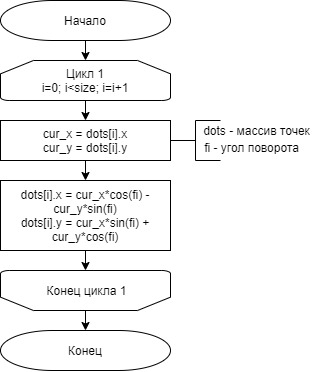
\includegraphics[scale=1]{linear.jpg}
		\caption{Схема последовательного алгоритма поворота фигуры}
		\label{fig:linear}
	\end{figure}

	\newpage
	
	На рисунках \ref{fig:paral}, \ref{fig:create} представлена схема распараллеливания алгоритма поворота фигуры.
	
	\begin{figure}[h]
		\centering
		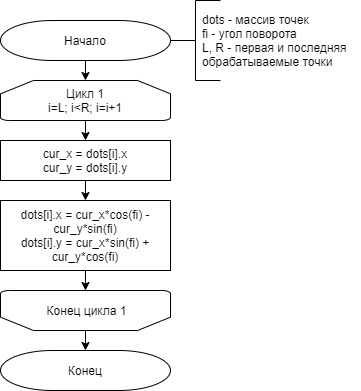
\includegraphics[scale=1]{paral.jpg}
		\caption{Схема многопоточного алгоритма поворота фигуры}
		\label{fig:paral}
	\end{figure}
	
	\newpage
	
	\begin{figure}[h]
		\centering
		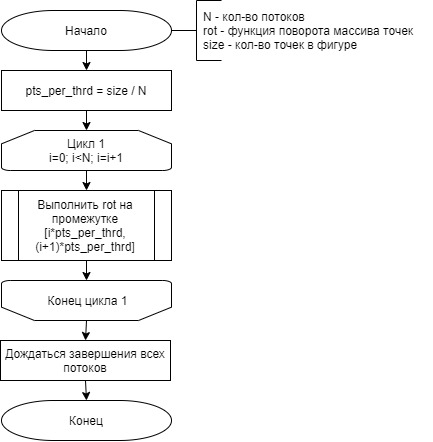
\includegraphics[scale=1]{create.jpg}
		\caption{Схема создания и запуска потоков}
		\label{fig:create}
	\end{figure}
	
	\section{Структуры данных}
	Для хранения фигуры будет использоваться структура, полями которой являются массив точек и количество точек (размер массива).
	
	Элементами массива точек в свою очередь будут также являться структуры, полями которых являются координаты этих точек по x и y.
	
	Все создаваемые потоки также будут храниться в массиве.
	
	\section{Тестирование и классы эквивалентности}
	Для проверки работоспособности ПО будет применяться функциональное тестирование.
	
	Классы эквивалентности:
	
	\begin{itemize}
		\item положительный угол поворота;
		\item отрицательный угол поворота;
		\item угол поворота - нулевой;
		\item угол поворота равен 360 градусам.
	\end{itemize}

	\section{Используемая память}
	Все вышеописанные массивы будут динамическими. В связи с этим, нужно будет контролировать проблемы с памятью, в частности при выделении памяти под массивы и её освобождении из-под них.
	
	Из всего вышесказанного следует, что количество памяти, необходимой алгоритмам, прямо пропорционально количеству точек фигуры и количеству потоков, используемых для распараллеливания.
	
	\section{Структура ПО}
	ПО будет состоять из набора функций:
	
	\begin{itemize}
		\item основная функция (main), работающая с меню;
		\item ввод исходных данных с клавиатуры;
		\item последовательный алгоритм поворота фигуры;
		\item параллельный алгоритм поворота фигуры;
		\item замеры процессорного времени.
	\end{itemize}
	
	\section{Вывод}
	На основе теоретических данных, полученные в аналитическом разделе были построены схемы исследуеммых алгоритмов. Также были описаны: структуры данных, используемые в алгоритмах, способы тестирования и классы эквивалентности, память, используемая алгоритмом, и структура ПО.
	
	\chapter{Технологическая часть}
	В этом разделе будут разработаны исходные коды последовательного и параллельного алгоритмов поворота фигуры.
	
	\section{Средства реализации}
	В качестве языка программирования для реализации данной лабораторной работы был выбран многопоточный язык С++. Данный выбор обусловлен моим желанием расширить свои знания в области применения данного языка.
	
	\section{Реализация алгоритмов}
	
	В листингах \ref{lin} - \ref{point} приведена реализация последовательного и параллельного алгоритмов поворота фигуры \cite{thread}.
	
	\begin{lstlisting}[label=lin,caption=Последовательный алгоритм поворота,language=C++]
	int rot(figure_t &fig, double fi, int fl)
	{
		double angle_pi = degrees_to_rad(fi);
		for (int i = 0; i < fig.n; ++i)
			point_rotate(fig.pts[i], angle_pi);
		return SUCCESS;
	}
	\end{lstlisting}

	\newpage
	
	\begin{lstlisting}[label=paral,caption=Параллельный алгоритм поворота,language=C++]
	void rot_part(figure_t& fig, double fi, int start_pt, int end_pt)
	{
		for (int i = start_pt; i < end_pt; i++)
			point_rotate(fig.pts[i], fi);
	}
	
	int rot_paral(figure_t& fig, double fi, int t_count)
	{
		auto* threads = new std::thread[t_count];
		
		double angle_pi = degrees_to_rad(fi);
		
		int pts_per_t = fig.n / t_count;
		int start_pt = 0, end_pt;
		for (int i = 0; i < t_count - 1; i++)
		{
			start_pt = i * pts_per_t;
			end_pt = (i + 1) * pts_per_t;
			threads[i] = std::thread(rot_part, std::ref(fig), angle_pi, start_pt, end_pt);
		}
		threads[t_count - 1] = std::thread(rot_part, std::ref(fig), angle_pi, (t_count - 1) * pts_per_t, fig.n);
		
		for (int i = 0; i < t_count; i++)
			threads[i].join();
		
		return SUCCESS;
	}
	\end{lstlisting}
	
	\begin{lstlisting}[label=point,caption=Функция поворота точки,language=C++]
	void point_rotate(point_t& point, double angle)
	{
		double tmp_x = point.x;
		point.x = point.x * cos(angle) - point.y * sin(angle);
		point.y = tmp_x * sin(angle) + point.y * cos(angle);
	}
	\end{lstlisting}

	\newpage
	
	В листинге \ref{cpu} представлена реализация замера процессорного времени \cite{process}.
	
	\begin{lstlisting}[label=cpu,caption=Функция замера процессорного времени,language=C++]
		#include <Windows.h>
		
		double getCPUTime()
		{
			FILETIME createTime;
			FILETIME exitTime;
			FILETIME kernelTime;
			FILETIME userTime;
			if (GetProcessTimes(GetCurrentProcess(),
			&createTime, &exitTime, &kernelTime, &userTime) != -1)
			{
				SYSTEMTIME userSystemTime;
				if (FileTimeToSystemTime(&userTime, &userSystemTime) != -1)
				return (double)userSystemTime.wHour * 3600.0 +
				(double)userSystemTime.wMinute * 60.0 +
				(double)userSystemTime.wSecond +
				(double)userSystemTime.wMilliseconds / 1000.0;
			}
		}
	\end{lstlisting}
	
	\section{Тестовые данные}
	
	В таблицах 3.1 - 3.2 приведены тестовые данные, на которых было протестированно разработанное ПО. Как видно из этой таблицы, все тесты были успешно пройдены, что означает, что программа работает правильно.
	
	\begin{table}[h]
		\label{tabular:func}
		\caption{Ожидаемый результат тестов}
		\begin{center}
			\begin{tabular}{ | c | c | c |}
				\hline
				\textbf{Точки} & \textbf{Угол поворота} & \textbf{Ожидаемый результат} \\ \hline
				[[1, 2], [2, 3], [3, 4], [4, 5]] & 90 &
				[[-2, 1], [-3, 2], [-4, 3], [-5, 4]]\\
				\hline
				
				[[1, 2], [2, 3], [3, 4], [4, 5]] & -90 &
				[[2, -1], [3, -2], [4, -3], [5, -4]]\\
				\hline
				
				[[1, 2], [2, 3], [3, 4], [4, 5]] & 360 &
				[[1, 2], [2, 3], [3, 4], [4, 5]] \\
				\hline
				
				[[1, 2], [2, 3], [3, 4], [4, 5]] & 0 &
				[[1, 2], [2, 3], [3, 4], [4, 5]] \\
				\hline
			\end{tabular}
		\end{center}
	\end{table}

	\begin{table}[h]
		\label{tabular:func2}
		\caption{Полученный результат тестов}
		\begin{center}
			\begin{tabular}{ | c | c | c |}
				\hline
				\textbf{Точки} & \textbf{Угол поворота} & \textbf{Полученный результат}\\ \hline
				[[1, 2], [2, 3], [3, 4], [4, 5]] & 90 &
				[[-2, 1], [-3, 2], [-4, 3], [-5, 4]] \\
				\hline
				
				[[1, 2], [2, 3], [3, 4], [4, 5]] & -90 &
				[[2, -1], [3, -2], [4, -3], [5, -4]] \\
				\hline
				
				[[1, 2], [2, 3], [3, 4], [4, 5]] & 360 &
				[[1, 2], [2, 3], [3, 4], [4, 5]] \\
				\hline
				
				[[1, 2], [2, 3], [3, 4], [4, 5]] & 0 &
				[[1, 2], [2, 3], [3, 4], [4, 5]] \\
				\hline
			\end{tabular}
		\end{center}
	\end{table}

	\newpage
	
	\section{Вывод}
	В данном разделе были разработаны исходные коды последовательного и параллельного алгоритмов поворота фигуры.
	
	\chapter{Исследовательская часть}
	В этом разделе будет проведён эксперимент для определения эффективности по времени работы каждого из разработанных алгоритмов.
	
	\section{Пример работы}
	
	Демонстрация работы программы приведена на рисунке 4.1.
	
	\begin{figure}[h]
		\begin{center}
			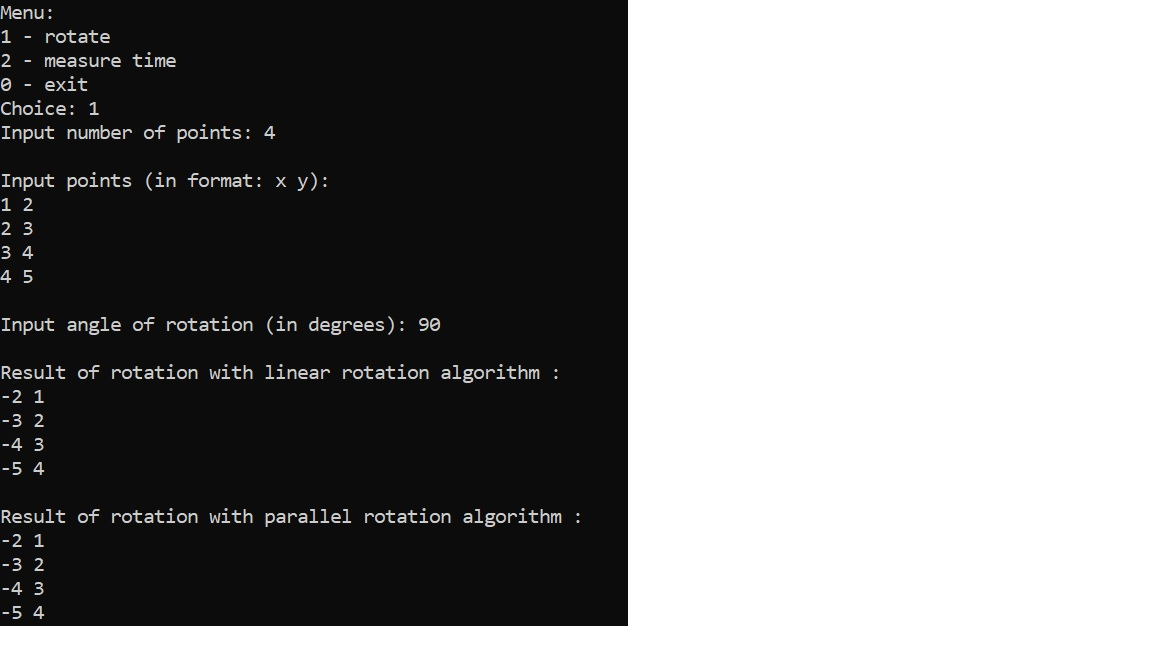
\includegraphics[scale=1]{example.jpg}
			\caption{Работа алгоритмов поворота фигуры.}
		\end{center}
	\end{figure}
	
	\section{Технические характеристики}
	
	Ниже приведеные технические характеристики устройства, на котором было проведенно тестирование ПО:
	
	\begin{itemize}
		
		\item Операционная система: Windows 10 64-bit Home \cite{home}.
		
		\item Оперативная память: 8 GB.
		
		\item Процессор: 11th Gen Intel(R) Core(TM) i3-1115G4 @ 3.00GHz
		\cite{i3}.
		
	\end{itemize}
	
	\section{Время выполнения алгоритмов}
	В таблицах 4.1 - 4.2 представлены замеры времени работы для каждого из алгоритмов.
	
	\begin{table} [h!]
		\caption{Время работы при различном кол-ве потоков (кол-во точек = 8000)}
		\begin{center}
			\begin{tabular}{|c c|} 
				\hline
				Кол-во потоков & Время (мс) \\  
				\hline
				1 & 1094 \\
				\hline
				2 & 594 \\
				\hline
				4 & 328 \\
				\hline
				8 & 279 \\
				\hline
				16 & 218 \\
				\hline
				32 & 207 \\
				\hline
			\end{tabular}
		\end{center}
	\end{table}

	\begin{table} [h!]
		\caption{Время работы при разном количестве точек}
		\begin{center}
			\begin{tabular}{|c c c|} 
				\hline
				Кол-во точек & 1 поток & 4 потока \\  
				\hline
				1000 & 109 & 107 \\
				\hline
				2000 & 203 & 168 \\
				\hline
				3000 & 344 & 209 \\
				\hline
				4000 & 438 & 228 \\
				\hline
				5000 & 546 & 265 \\
				\hline
				6000 & 641 & 327 \\
				\hline
				7000 & 766 & 406 \\
				\hline
				8000 & 891 & 484 \\
				\hline
			\end{tabular}
		\end{center}
	\end{table}
	
	\begin{figure}[h!]
		\begin{center}
			\begin{tikzpicture}
				\begin{axis}[
					legend pos = north west,
					xlabel=кол-во потоков,
					ylabel=милисекунды,
					minor tick num = 1,
					grid = both,
					major grid style = {lightgray},
					minor grid style = {lightgray!25},
					xtick distance = 10,
					width = 0.9\textwidth,
					height = 0.5\textwidth]
					
					\addplot[
					blue,
					semithick,
					mark = x,
					mark size = 3pt,
					thick,
					] file {difThrds.txt};
					
					\legend{
						Кол-во точек = 8000
					}
				\end{axis}
			\end{tikzpicture}
		\end{center}
		\caption{Параллельный алгоритм при различном кол-ве потоков}
	\end{figure}
	
	\begin{figure}[h!]
		\begin{center}
			\begin{tikzpicture}
				\begin{axis}[
					legend pos = north west,
					xlabel=кол-во точек,
					ylabel=милисекунды,
					minor tick num = 1,
					grid = both,
					major grid style = {lightgray},
					minor grid style = {lightgray!25},
					xtick distance = 1000,
					width = 0.9\textwidth,
					height = 0.5\textwidth]
					
					\addplot[
					blue,
					semithick,
					mark = x,
					mark size = 3pt,
					thick,
					] file {1thrd.txt};
					
					\addplot[
					red,
					semithick,
					mark = *,
					] file {4thrds.txt};
					
					\legend{
						1 поток,
						4 потока
					}
				\end{axis}
			\end{tikzpicture}
		\end{center}
		\caption{Сравнение времени работы алгоритмов при разном кол-ве точек}
	\end{figure}

	\newpage
	
	\section{Вывод}
	
	В результате проведенного эксперимента можно сделать вывод, что использование многопоточности однозначно может дать существенный выигрыш по времени работы алгоритма. Так, алгоритм с 4 потоками на 8000 точек эффективнее однопоточного примерно на 45,7\%.
	
	При этом на небольшом количестве точек использование многопоточности неэффективно, т. к. в таком случае накладные расходы на создание потоков превышают выигрыш от использования распараллеливания. Например, на 1000 точек, как видно из эксперимента, однопоточный алгоритм практически не отличается по времени от многопоточного.
	
	\chapter*{Заключение}
	\addcontentsline{toc}{chapter}{Заключение}
	
	В ходе проделанной работы были изучены и реализованы однопоточный и многопоточный алгоритмы поворота фигуры. 
	
	Экспериментально было подтверждено различие по временной эффективности этих алгоритмов на материале замеров процессорного времени выполнения реализации на варьирующемся количестве точек. Так, многопоточный алгоритм на существенных размерах данных работает значительно быстрее однопоточного (например, алгоритм с 4 потоками на 8000 точек эффективнее по времени однопоточного примерно на 45,7\%).
	
	При этом на малом количестве точек эта разница незаметна или даже, наоборот, многопоточный алгоритм начинает терять свою эффективность, так как накладные расходы на создание потоков в таком случае превышают выигрыш распараллеливания.
	
	\addcontentsline{toc}{chapter}{Список литературы}
	
	\bibliographystyle{utf8gost705u}  % стилевой файл для оформления по ГОСТу
	
	\bibliography{biblio}          % имя библиографической базы (bib-файла)
	
\end{document}
